\chapter{Lunar Lander}
In questo capitolo cercheremo di risolvere l'ambiente Lunar Lander analizzato nella Sezione \ref{sec:lunalander}.

Come criterio per verificare l'obiettivo si è considerato il raggiungimento in modo consistente di una returns per episodio di 200 punti. Il grafico che ci farà osservare questo comportamento è quello che mette in evidenza la somma delle reward per ogni epoca; vista l'elevata rumorosità, è stato rappresentato con un Time Weighted EMA con un fattore di 0{,}95.

%%%%%%%%%%%%%%%%%%%%%%%%%%%%%%%%%%%%%%%%%%%%%%%%
\section{Baseline}
Per cercare di risolvere l'ambiente utilizzando gli stessi metodi di Cart Pole, sono stati eseguiti tre esperimenti usando le tre baseline definite nel Capitolo \ref{chap:cartpole}: senza baseline, con la standardizzazione e con l'approssimazione della state-value function tramite una rete neurale. Siccome l'ambiente è più complesso rispetto a Cart Pole, ho deciso di addestrare l'agente per 5000 episodi, contro le 3000 usate in precedenza.

\myskip

Come si può osservare dai risultati in Figura \ref{fig:lunarbaseline}, mentre risolvere Cart Pole era banale, adesso il compito è più complesso. Si può notare che la soluzione senza baseline fa molta fatica, e in praticamente nessun episodio è stata raggiunta una somma dei rewards superiore a 200. Con la standardizzazione e la state-value function la situazione migliora: ci sono degli episodi in cui l'ambiente è risolto, ma questo succede in modo non stabile e quindi il risultato non ci soddisfa. Usare più episodi (20K) non migliora l'addestramento, come si vede in Figura \ref{fig:lunarstatelong}; dobbiamo quindi cercare di cambiare un po' le cose per cercare una soluzione più soddisfacente.

Come osservato nel capitolo precedente possiamo notare come la soluzione con la baseline che approssima la state-value function è più stabile.

\begin{figure}[htbp]
    \centering
    \begin{subfigure}{0.45\textwidth}
        \centering
        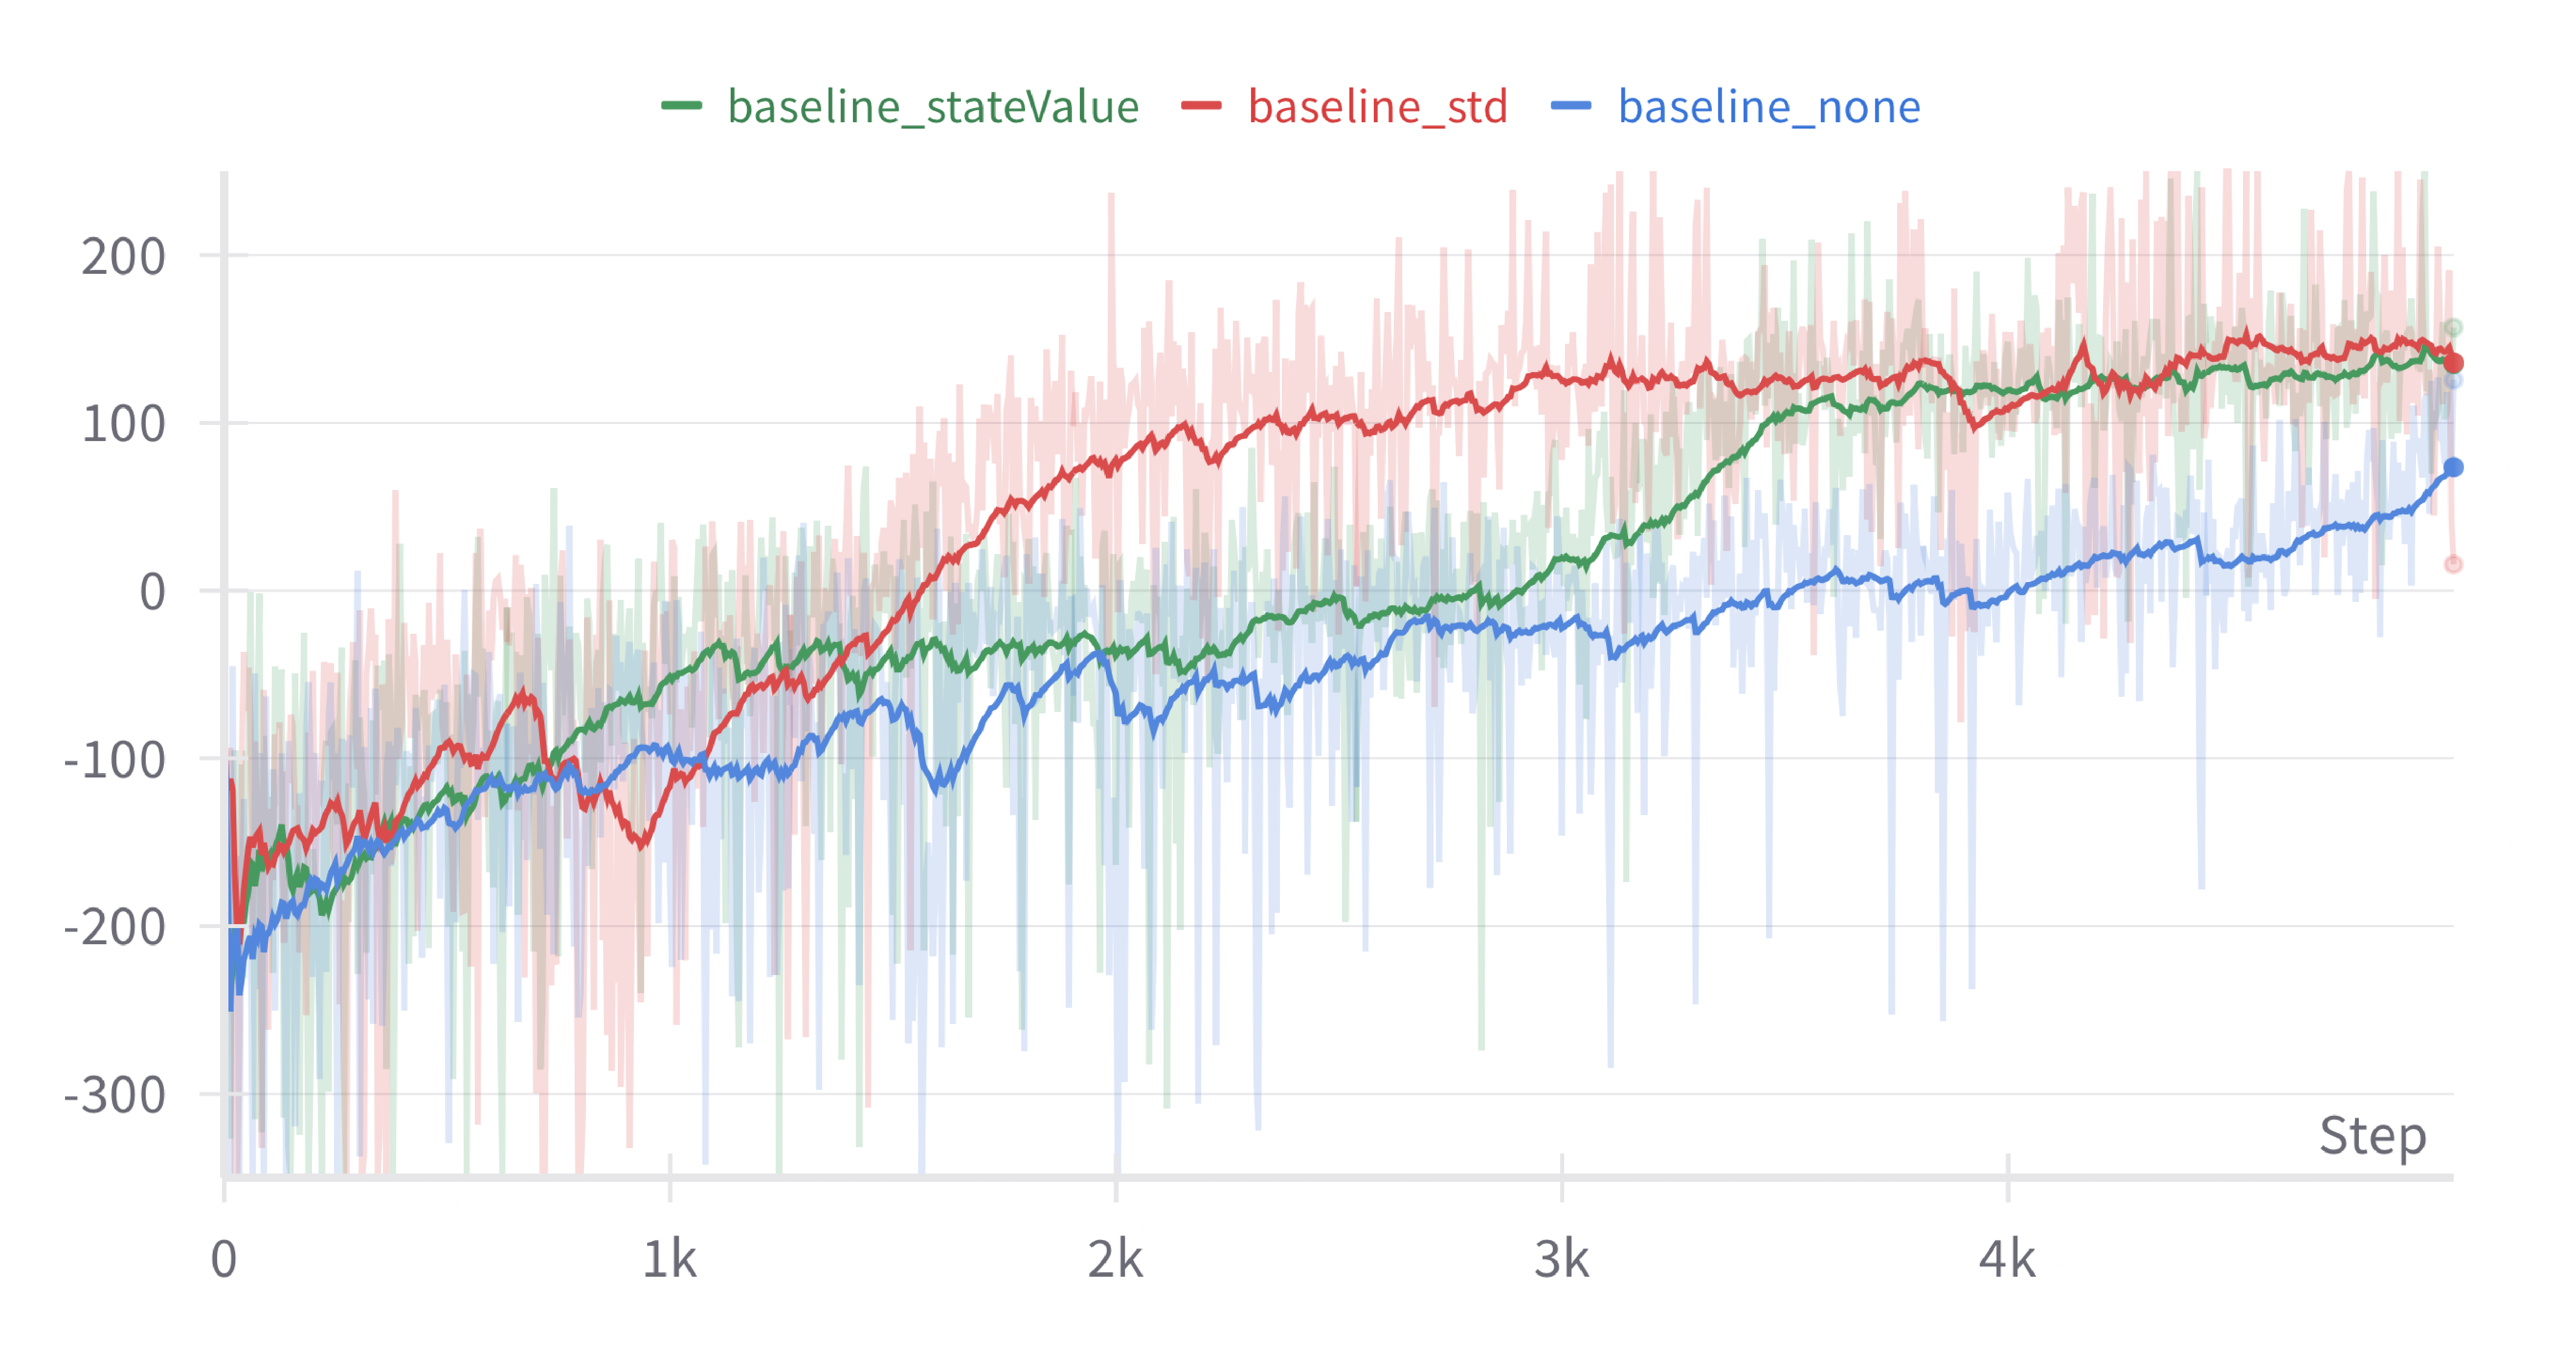
\includegraphics[width=\textwidth]{immages/4-lunar lander/returs_baseline.pdf}
        \caption{Tre baseline.}
        \label{fig:lunarbaseline}
    \end{subfigure}
    \hfill
    \begin{subfigure}{0.45\textwidth}
        \centering
        \includegraphics[width=\textwidth]{immages/4-lunar lander/long.pdf}
        \caption{Baseline con state-value function.}
        \label{fig:lunarstatelong}
    \end{subfigure}
\end{figure}

%%%%%%%%%%%%%%%%%%%%%%%%%%%%%%%%%%%%%%%%%%%%%%%%
\section{Architettura rete neurale}
Nel seguito i vari esperimenti sono stati eseguiti con la state-value function baseline. In questo capitolo vediamo come è stata cambiata la rete che approssima la policy e la state-value function; ricordiamo che queste due hanno la stessa architettura.

Sono state provate varie architetture: la profondità è di tre layer interni tutti con lo stesso numero di neuroni; in un caso 32, in un altro 64 e nell'ultimo 128. Visto il contesto molto stocastico, sono stati fatti tre esperimenti per ogni architettura, ognuno dei quali è stato eseguito per 10000 episodi.

\myskip

Osserviamo i vari esperimenti fatti. Come si può notare dalle Figure \ref{fig:architetture}, all'aumentare della complessità della rete aumenta anche la differenza di risultati da un esperimento all'altro. Si può anche osservare che una rete più complessa sembra essere più promettente rispetto a una più semplice nell'arrivare al risultato, cioè ai 200 punti per episodio.

\begin{figure}[htbp]
    \centering
    \begin{subfigure}{0.3\textwidth}
        \centering
        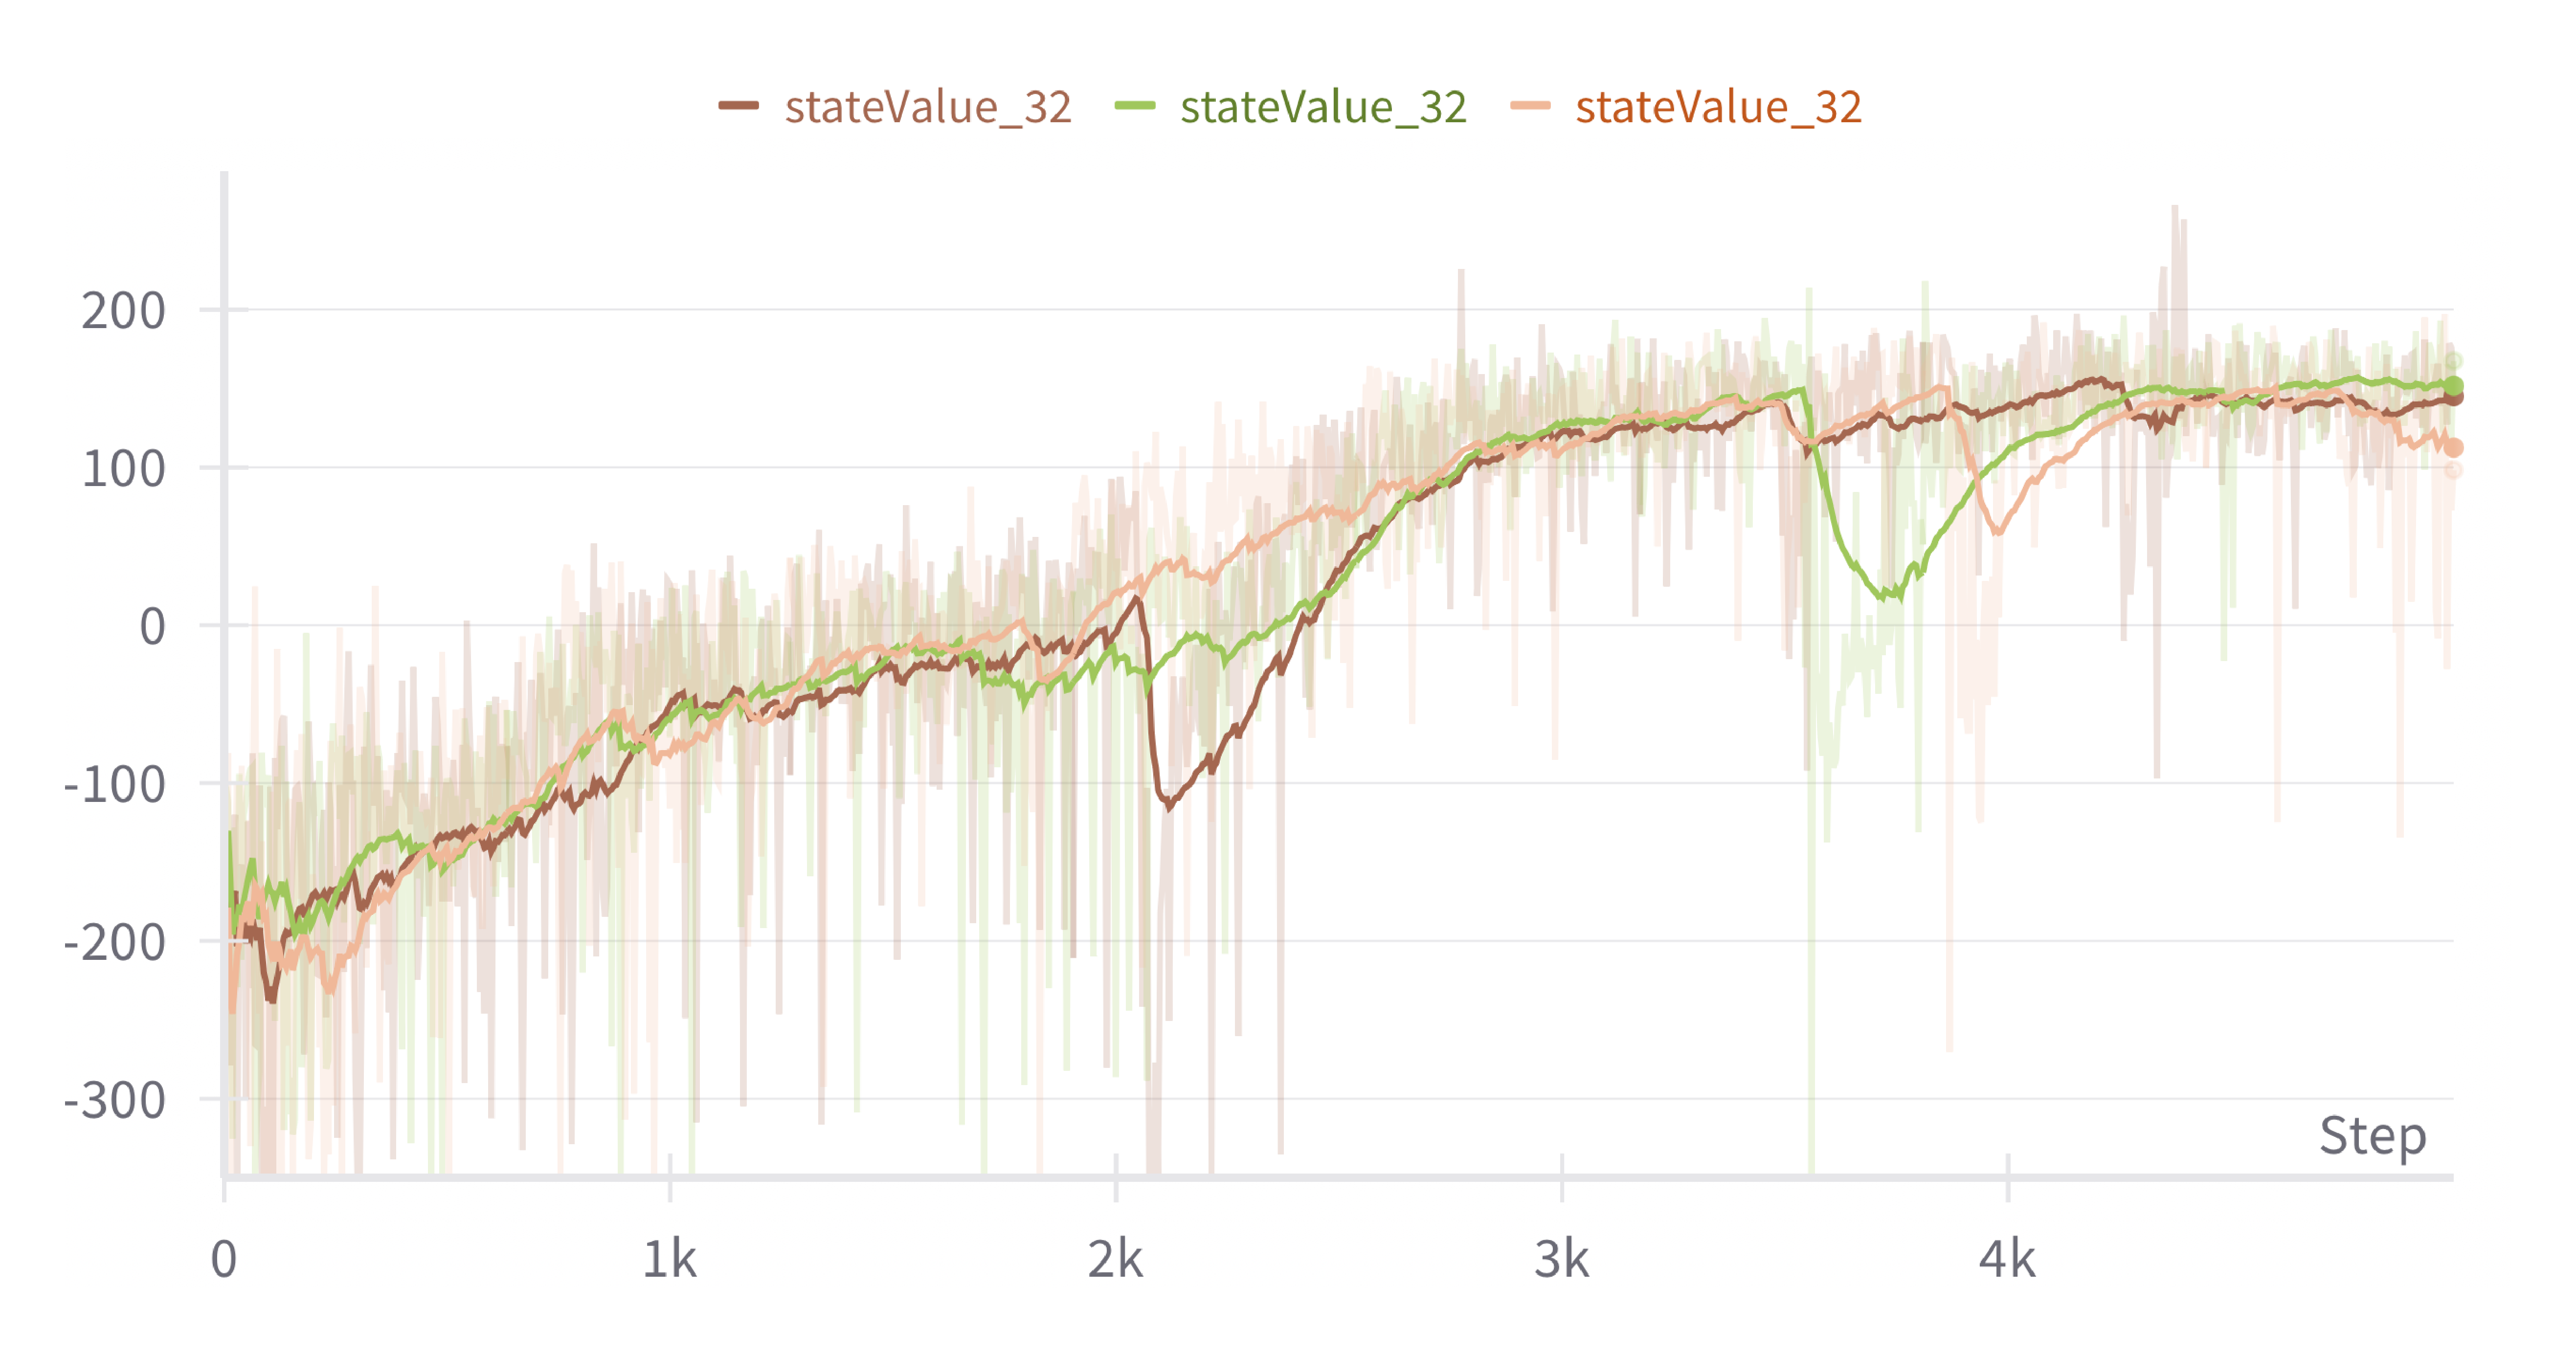
\includegraphics[width=\textwidth]{immages/4-lunar lander/32.pdf}
        \caption{Tre hidden layer da 32 neuroni.}
        \label{fig:32}
    \end{subfigure}
    \hfill
    \begin{subfigure}{0.3\textwidth}
        \centering
        \includegraphics[width=\textwidth]{immages/4-lunar lander/64.pdf}
        \caption{Tre hidden layer da 64 neuroni.}
        \label{fig:64}
    \end{subfigure}
    \hfill
    \begin{subfigure}{0.3\textwidth}
        \centering
        \includegraphics[width=\textwidth]{immages/4-lunar lander/128.pdf}
        \caption{Tre hidden layer da 128 neuroni.}
        \label{fig:128}
    \end{subfigure}
    \caption{Varie architetture.}
    \label{fig:architetture}
\end{figure}

%%%%%%%%%%%%%%%%%%%%%%%%%%%%%%%%%%%%%%%%%%%%%%%%
\section{Step scheduler}
Per cercare di migliorare la stabilità dell'addestramento è stato introdotto uno scheduler per i due ottimizzatori delle reti che approssimano la policy e la state-value function. Lo scheduler in questione è uno dei più semplici, cioè \texttt{StepLR}: ogni 1500 episodi il learning rate è decrementato di un fattore di 0{,}9.

I risultati ottenuti sono quelli mostrati in Figura \ref{fig:steplr}. Come si può osservare, la stabilità è migliorata leggermente, soprattutto per il modello più complesso. Nonostante questo, i risultati non sono del tutto soddisfacenti per quanto riguarda le performance.

\begin{figure}[htbp]
    \centering
    \begin{subfigure}{0.3\textwidth}
        \centering
        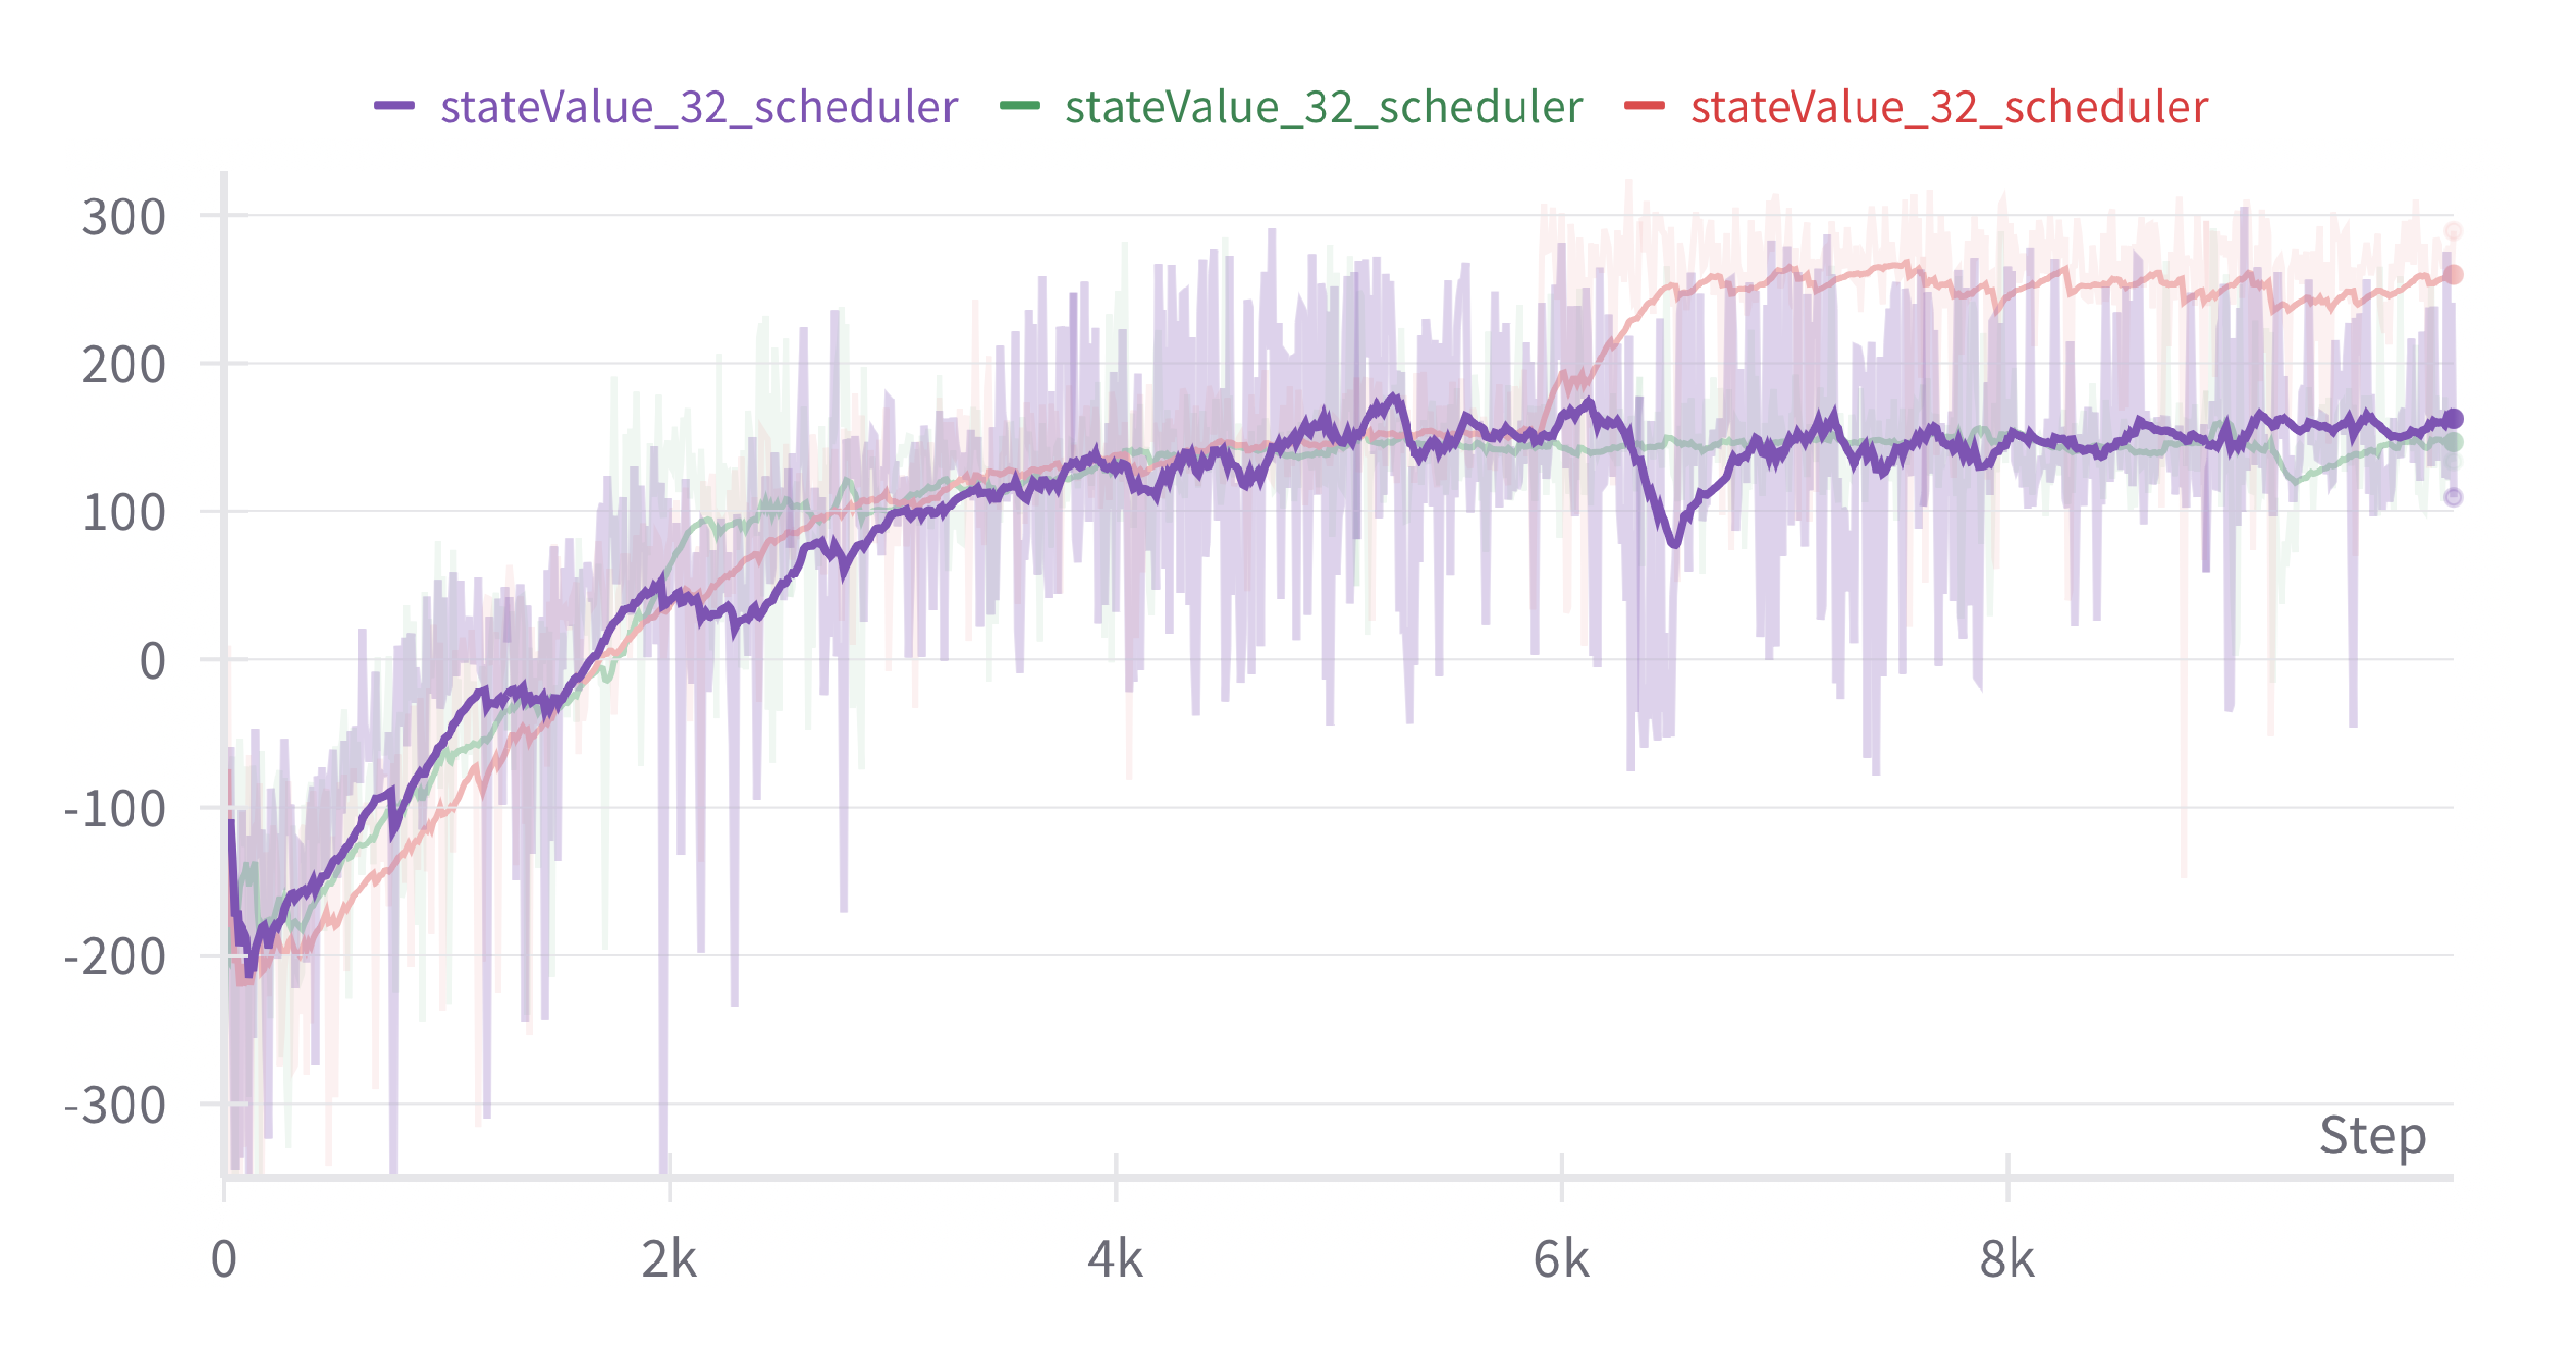
\includegraphics[width=\textwidth]{immages/4-lunar lander/32_scheduler.pdf}
        \caption{Tre hidden layer da 32 neuroni.}
    \end{subfigure}
    \hfill
    \begin{subfigure}{0.3\textwidth}
        \centering
        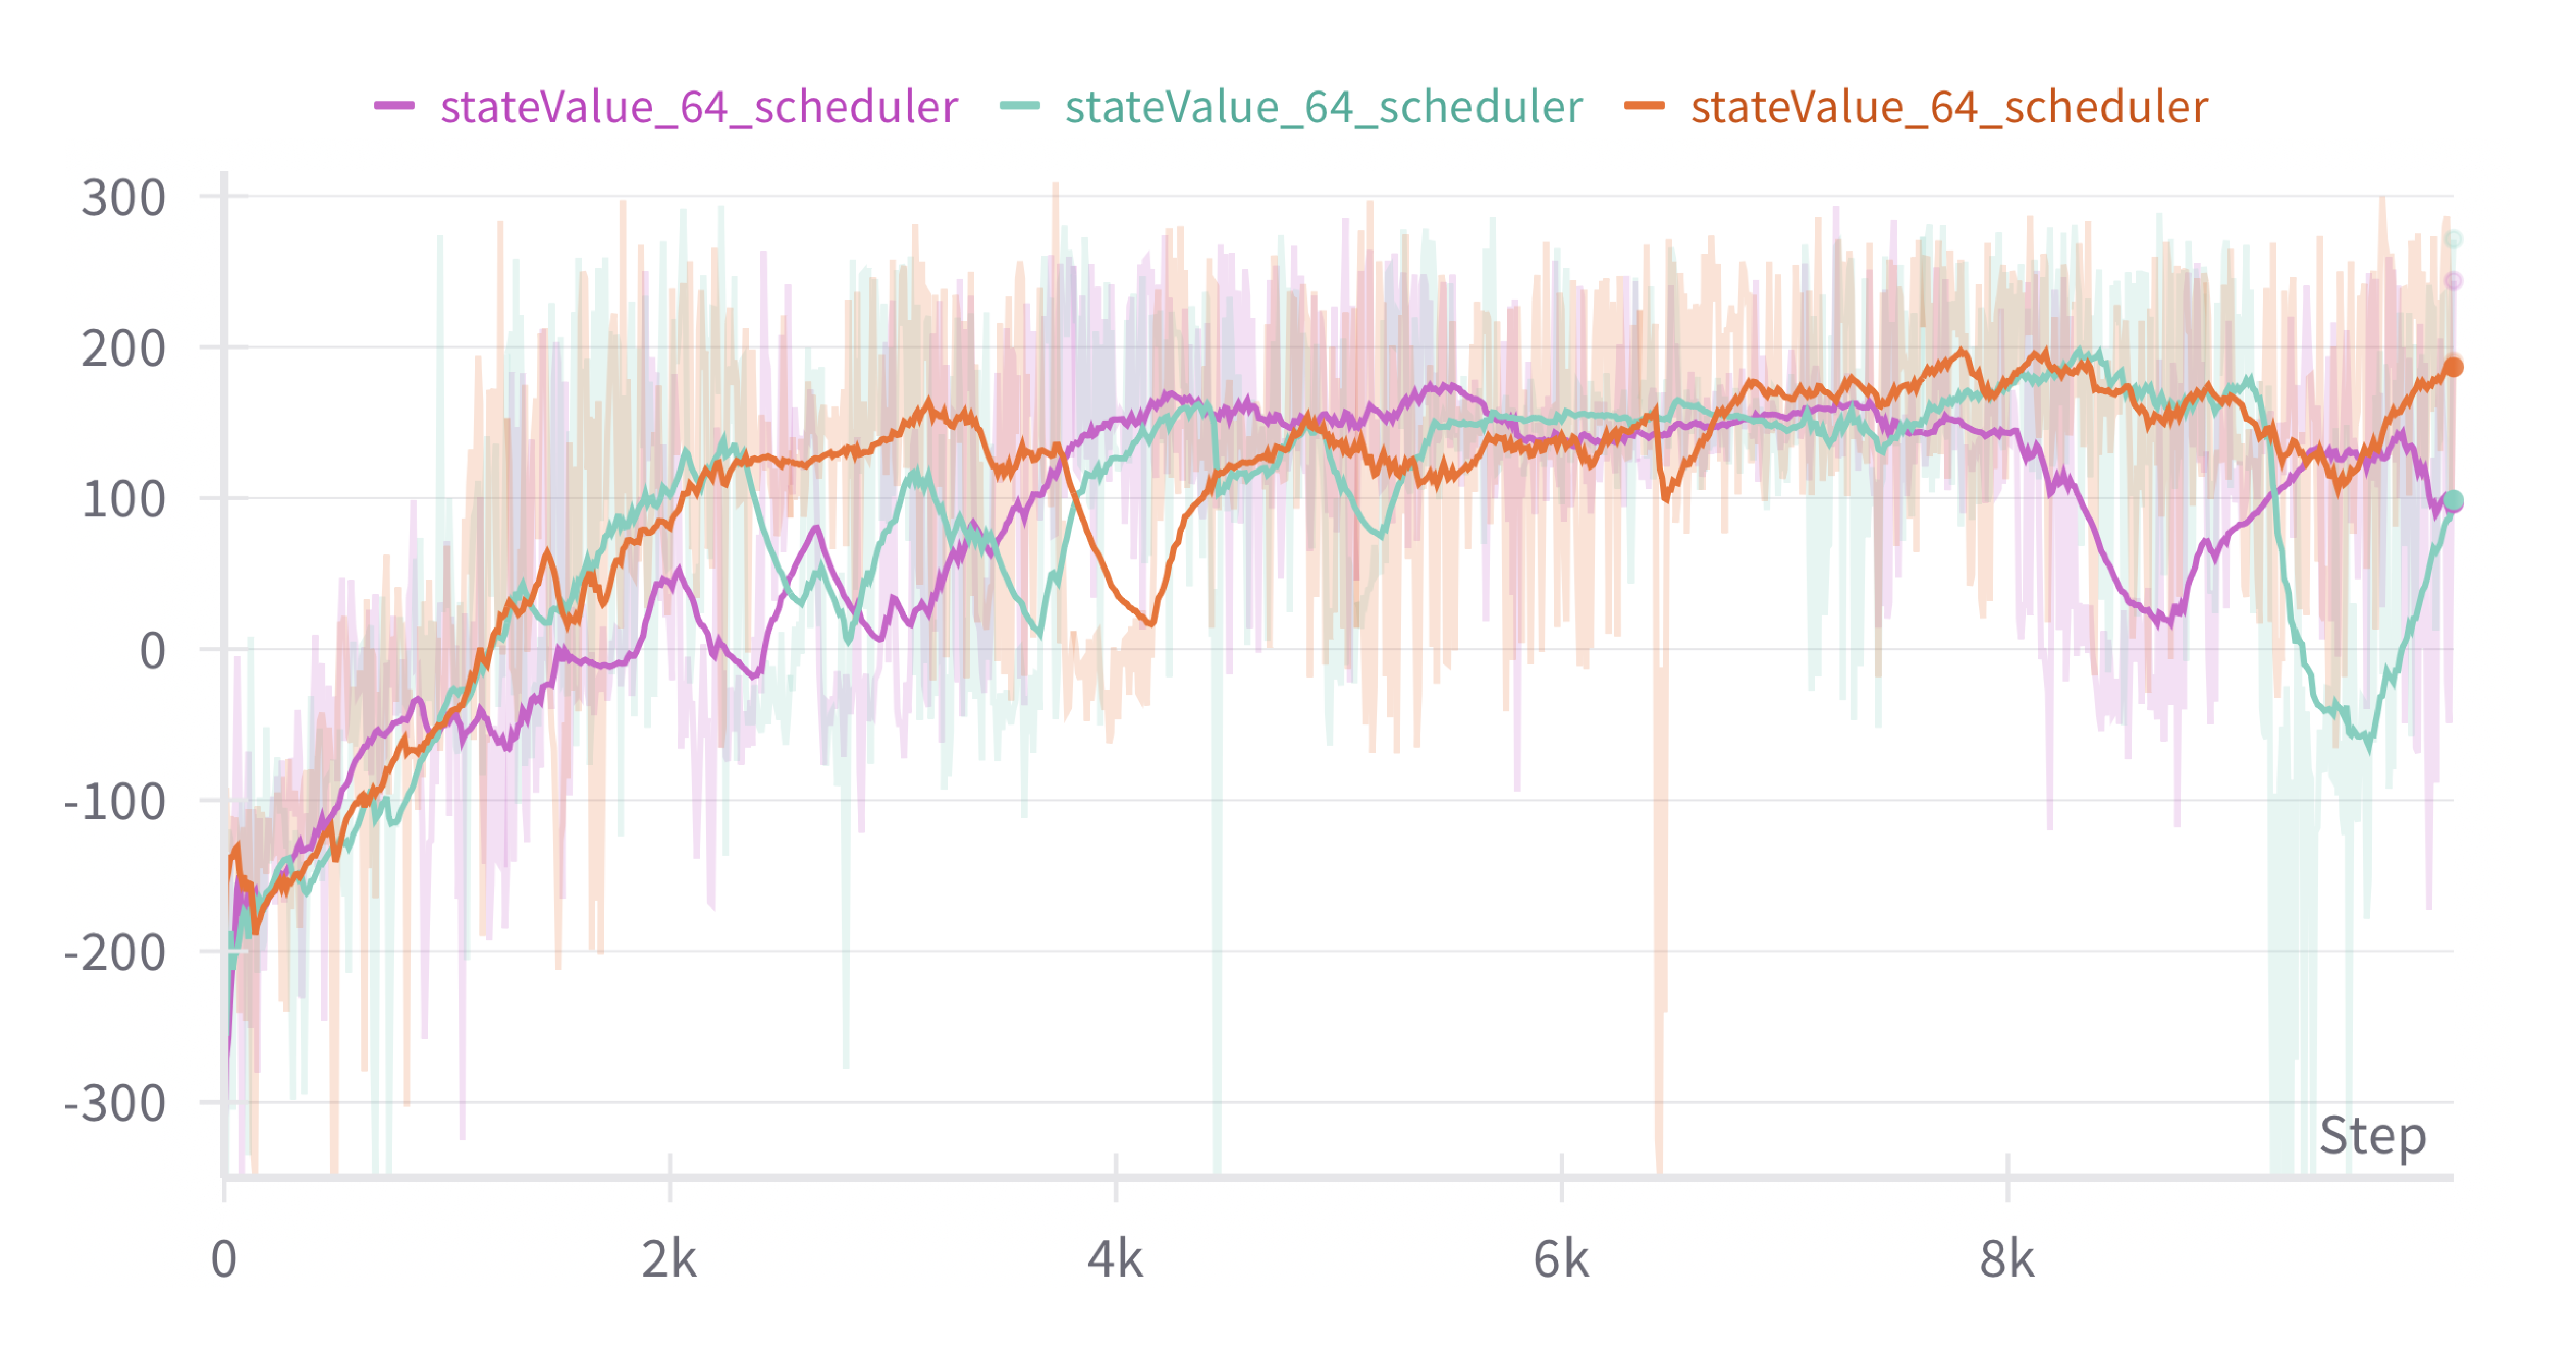
\includegraphics[width=\textwidth]{immages/4-lunar lander/64_scheduler.pdf}
        \caption{Tre hidden layer da 64 neuroni.}
    \end{subfigure}
    \hfill
    \begin{subfigure}{0.3\textwidth}
        \centering
        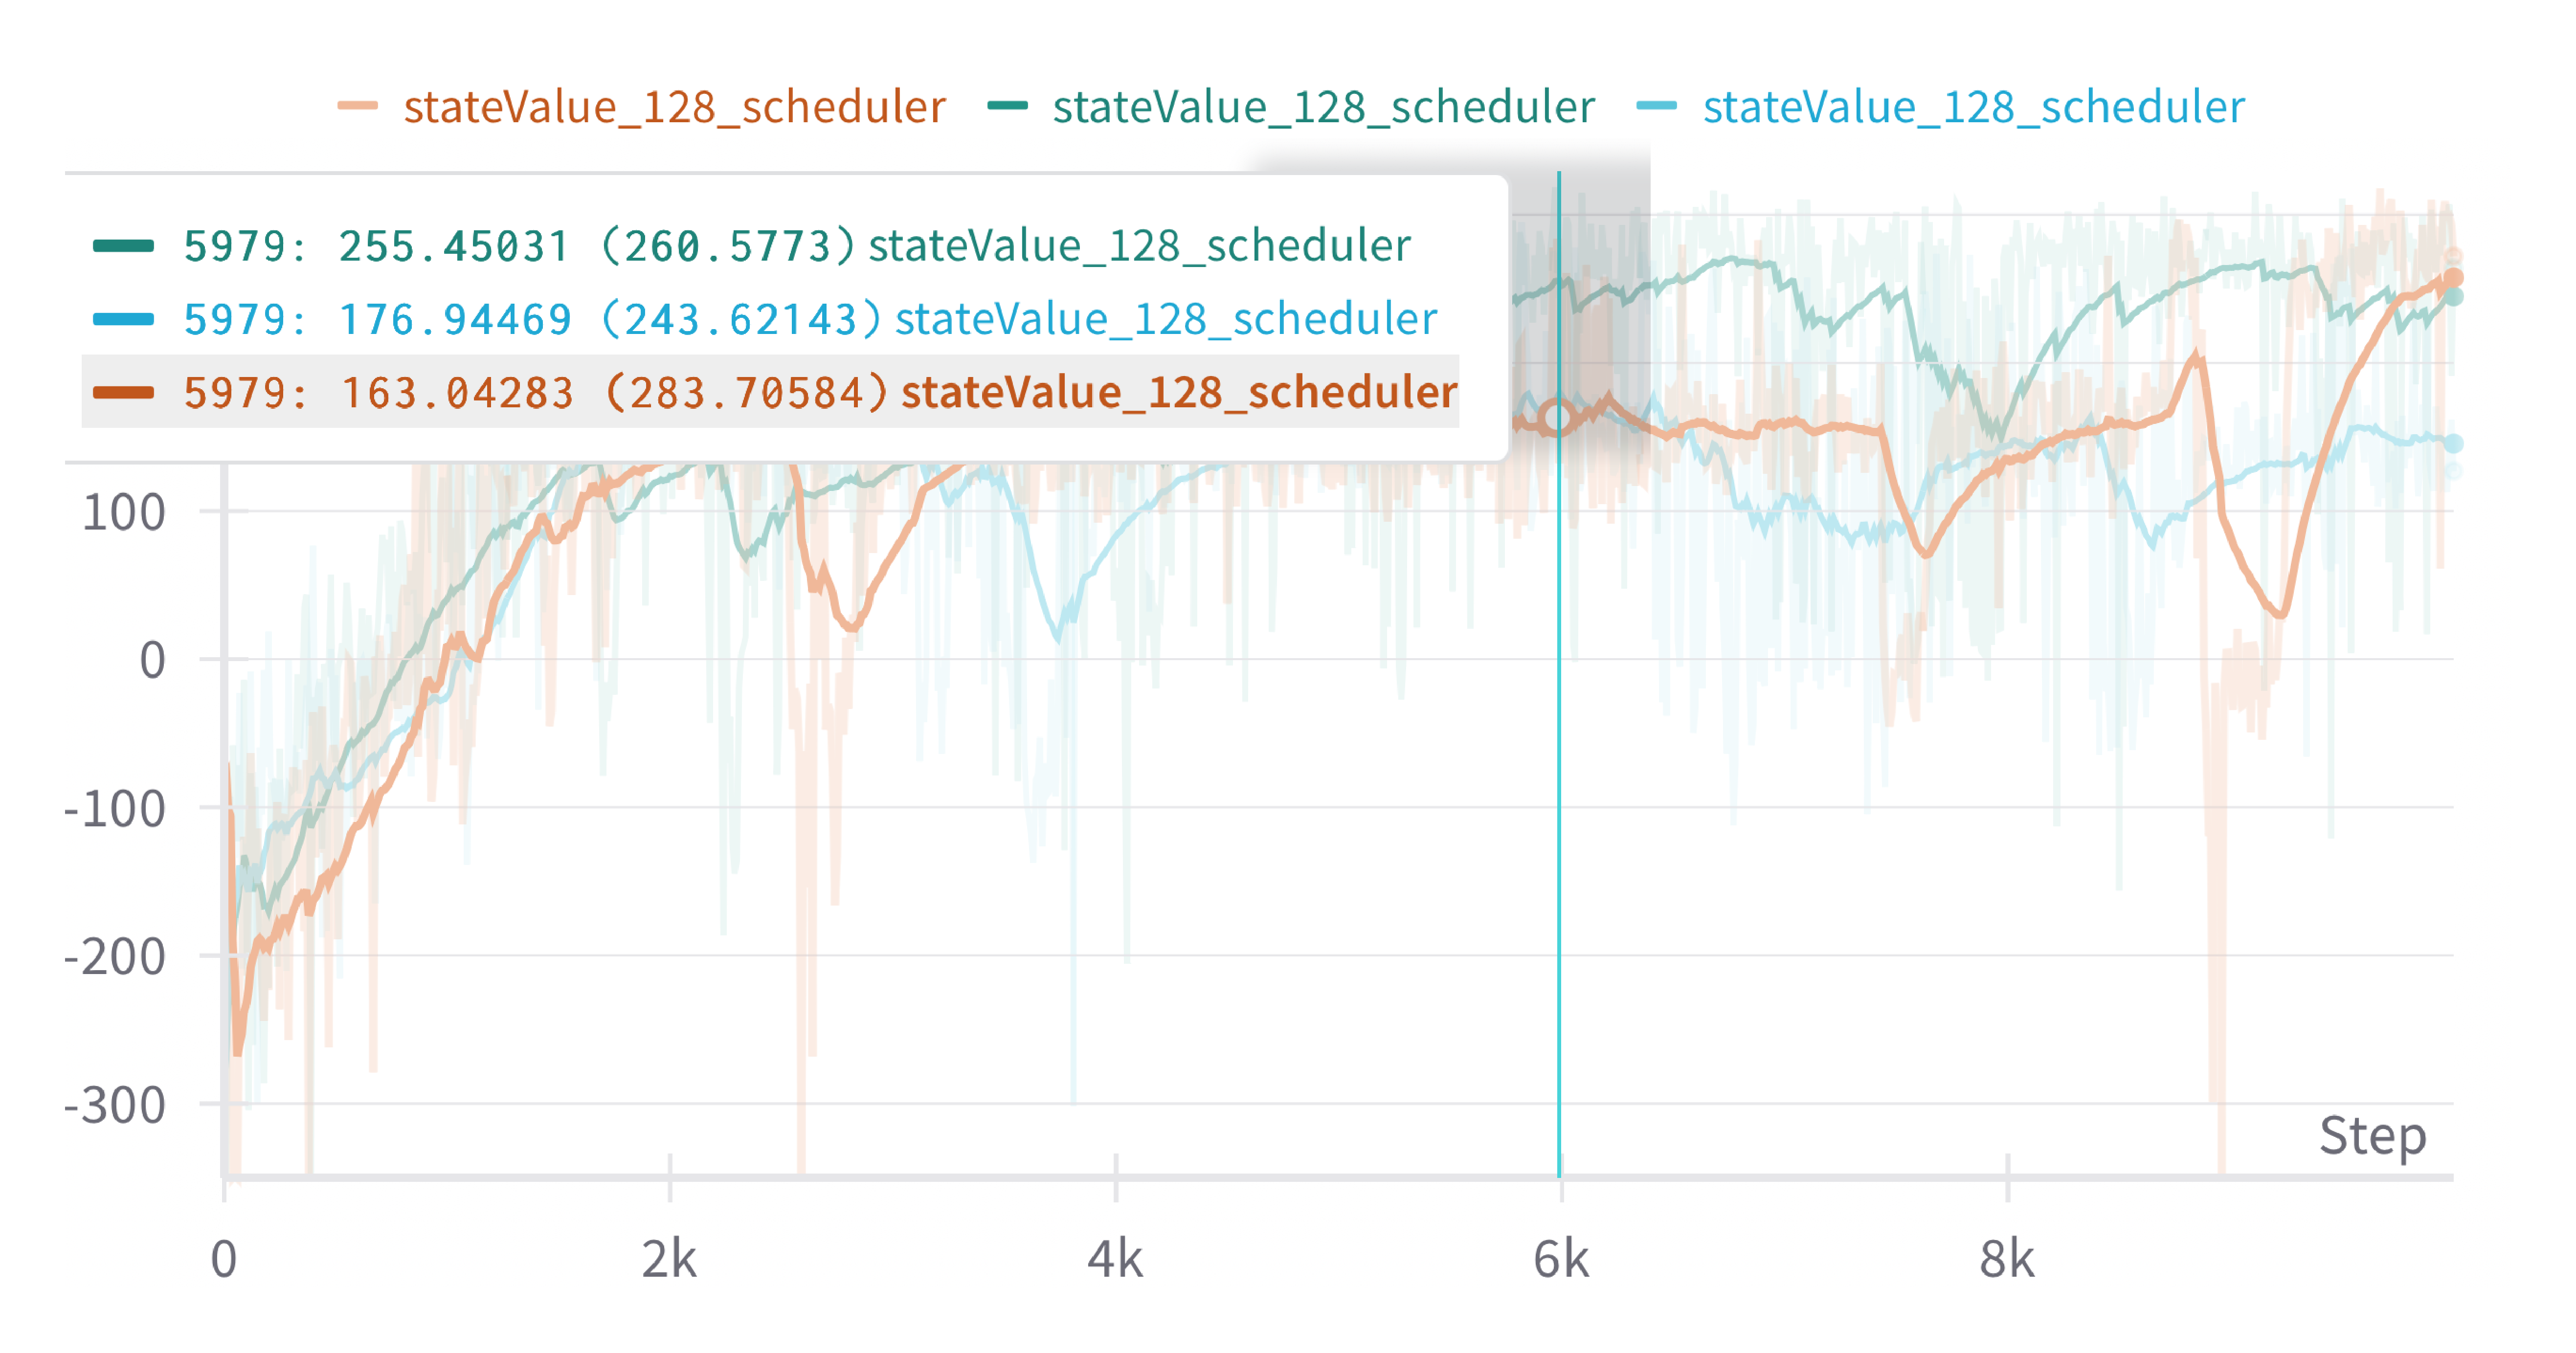
\includegraphics[width=\textwidth]{immages/4-lunar lander/128_scheduler.pdf}
        \caption{Tre hidden layer da 128 neuroni.}
    \end{subfigure}
    \caption{Scheduler StepLR.}
    \label{fig:steplr}
\end{figure}

%%%%%%%%%%%%%%%%%%%%%%%%%%%%%%%%%%%%%%%%%%%%%%%%
\section{Gradient clipping}
Il metodo che forse ha dato il miglioramento più evidente è stato quello di limitare la norma dei gradienti per evitare il fenomeno dell'exploding gradient, molto comune nel reinforcement learning.

Sono stati testati tre valori per il massimo delle norme: 2, 5 e 10. Come si può notare dalla Figura \ref{fig:norm}, i risultati migliori li abbiamo quando cerchiamo di limitare maggiormente la norma dei gradienti; questo ci fa capire quanto sia importante il fenomeno dell'exploding gradient in questo contesto.

Con questo risultato si può dire, anche osservando la visualizzazione, che l'ambiente è risolto.

\begin{figure}[htbp]
    \centering
    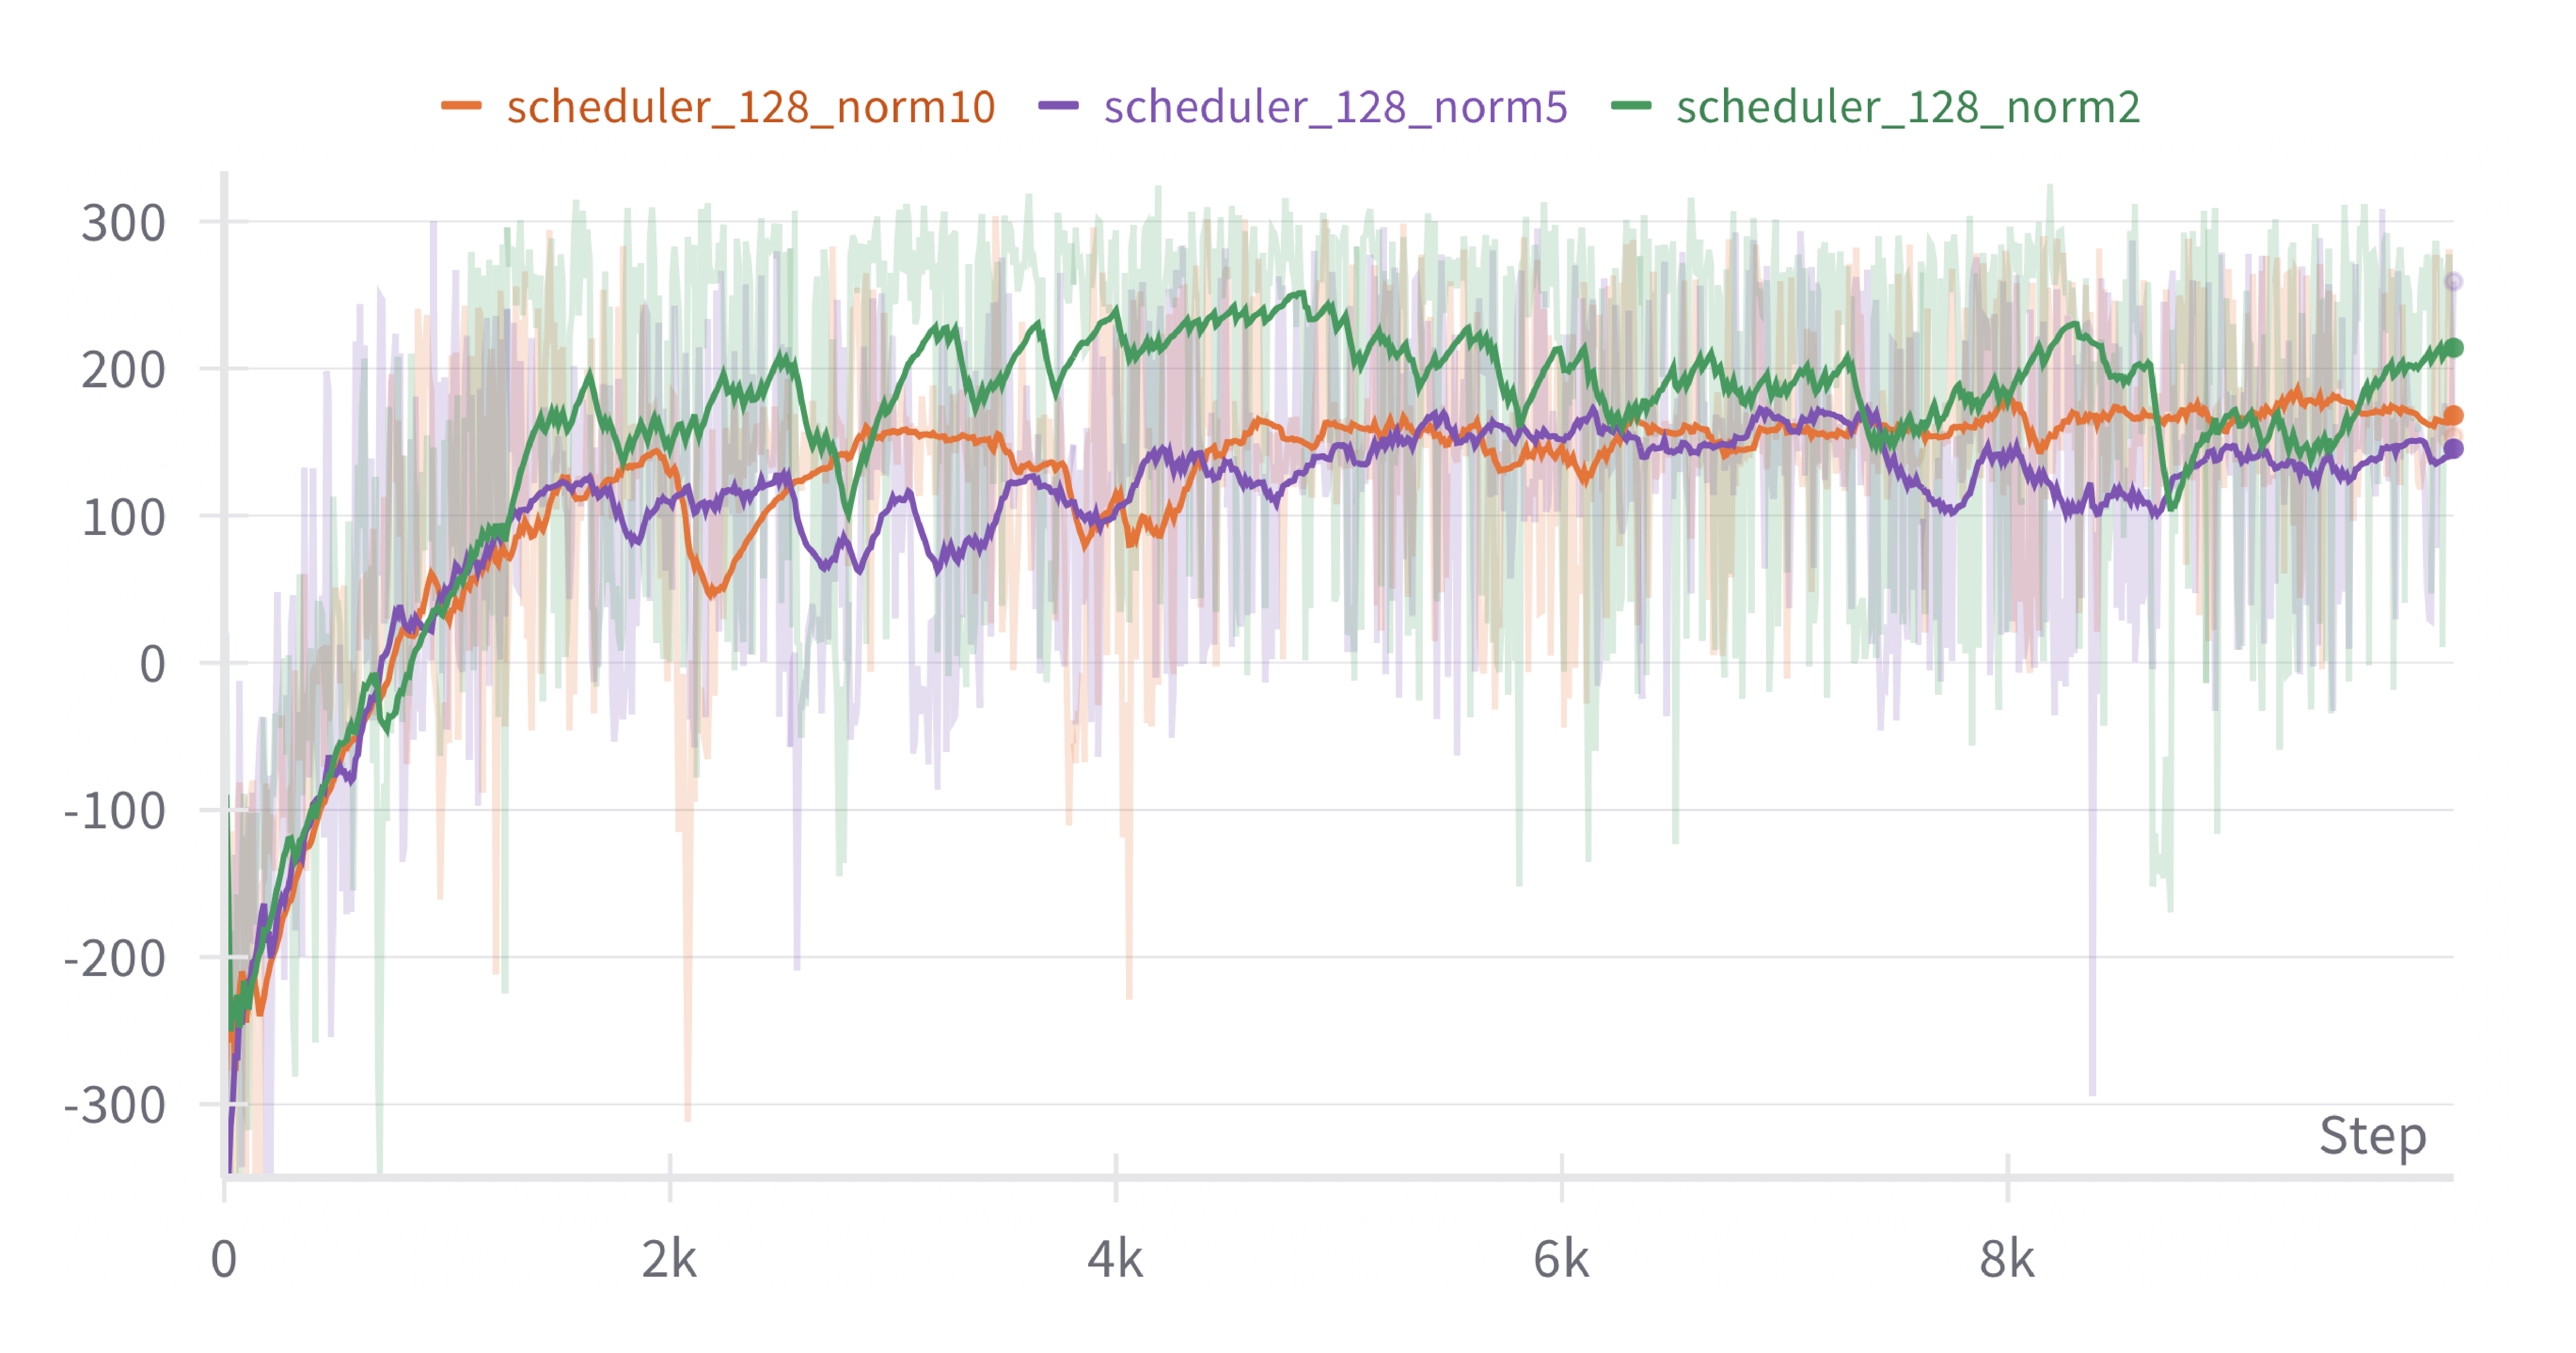
\includegraphics[width=.9\textwidth]{immages/4-lunar lander/norm_result.pdf}
    \caption{Risultati con gradient clipping.}
    \label{fig:norm}
\end{figure}